\documentclass{IEEEtran}
\usepackage{mathtools}
\usepackage{graphicx}
\usepackage{amssymb}
\usepackage{amsmath}
\usepackage{pythonhighlight}
\usepackage[utf8]{inputenc}
\usepackage{fancyhdr}
\usepackage{pythonhighlight}
\usepackage{changepage}
\usepackage{slashbox}
\usepackage{floatrow}
\usepackage{listings}
\usepackage{derivative}
\usepackage[hidelinks]{hyperref}
\usepackage{fontawesome}
\usepackage{caption}
\usepackage{subcaption}
\usepackage[sorting=none,style=ieee]{biblatex}
\usepackage{cleveref}
\usepackage{algorithm}
\usepackage{algpseudocode}
\usepackage{physics}
\usepackage{lipsum}
\usepackage{titlesec}



\addbibresource{report.bib}
\title{Analysis of TransUNet}
\author{Kutay Ugurlu}

\begin{document}
\maketitle
\begin{abstract}
    Medical image segmentation is a cruical part of developing healthcare systems, not only in imaging in the covnentional sense, but also in electrical source imaging of brain and heart \cite{gonzalez2020ecgi}. So far, U-Net\cite[text]{ronneberger2015u} has become ubiquitous in the medical image segmentation tasks due to its recognized performance. However, the intrinsic features of convolutional neural networks(CNNs) that extract the local features of the spatial region in the image, the architecture exhibits some limitations finding the long-range patterns. On the other hand, transformers, that were developed for sequence-to-sequence predictions, are able to recognise the global patterns via the utilization of attention mechanism \cite{vaswani2017attention}. Chen, \textit{et al.}, propose a hybrid CNN-Transformer network called TransUNet in their study  \cite{chen2021transunet} to tackle the problem of medical image segmentation exploiting both local and global dependencies in the images.
    In this project, the aforesaid study is analyzed and a series of experimentation is conducted whose results are available online at the forked repository: \href{https://github.com/kutay-ugurlu/TransUNet_Analysis}{https://github.com/kutay-ugurlu/TransUNet\_Analysis}. 
\end{abstract}
\section{Introduction}

Image segmentation is a semantic segmentation task where each of the pixels (or voxels) are assigned a class corresponding to the object that they represent. The medical image segmentation has been an particular interest of researchers for diagnosis, treatment and even prognosis, in different fields. Given the small size of medical datasets available, the segmentation is a challenging task \cite{ren2019brain}. Furthermore, especially in human imaging, the segmentation boundaries need to be precise to make reliable decisions on the data. Hence, a model has to be trained to seperate the organ and physiological boundaries succesfully with a high spatial resolution, as in \Cref{fig:brainseg}, while also having the capability to generalize to other data distributions it may be fed. 

\begin{figure}[h]
    \centering
    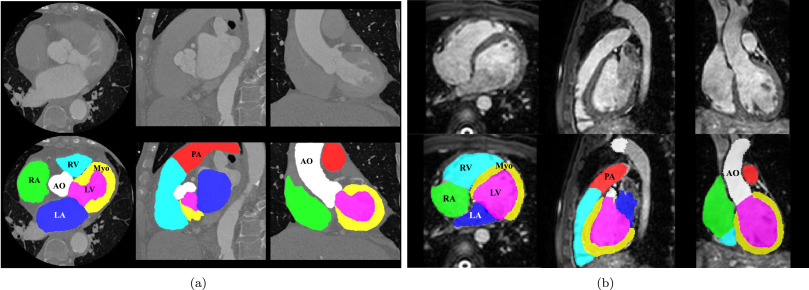
\includegraphics[width=\textwidth]{img/heartseg1.jpg}
    \caption{Whole Heart Segmentation \cite{ZHUANG2019101537}}\label{fig:heartseg}
    \end{figure}

\begin{figure}[h]
    \centering
    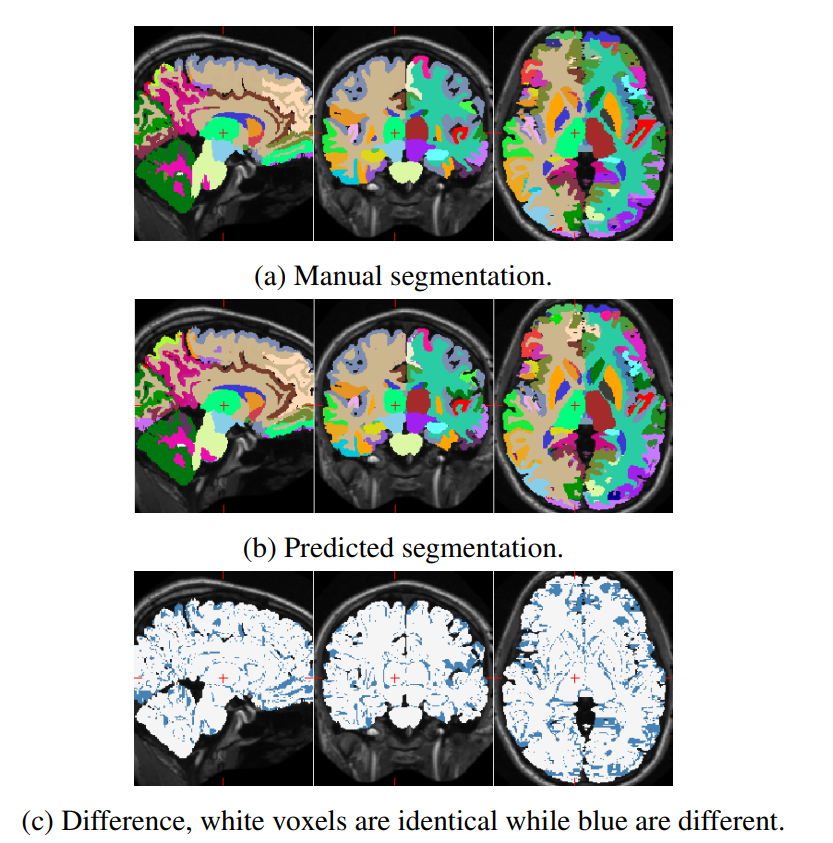
\includegraphics[width=\textwidth]{img/brainseg.png}
    \caption{Whole Brain Segmentation \cite{de2015deep}}\label{fig:brainseg}
    \end{figure}


To improve both the local and global pattern recognition capability, the authors of \cite{chen2021transunet} proposes a hybrid network whose components are going to be analyzed individually in the following sections. 

\section{Theory}

\subsection{U-Net}
U-Net is a convolutional neural network that utilizes certain modifications compared to its predecessors. 

\begin{figure}[h]
\centering
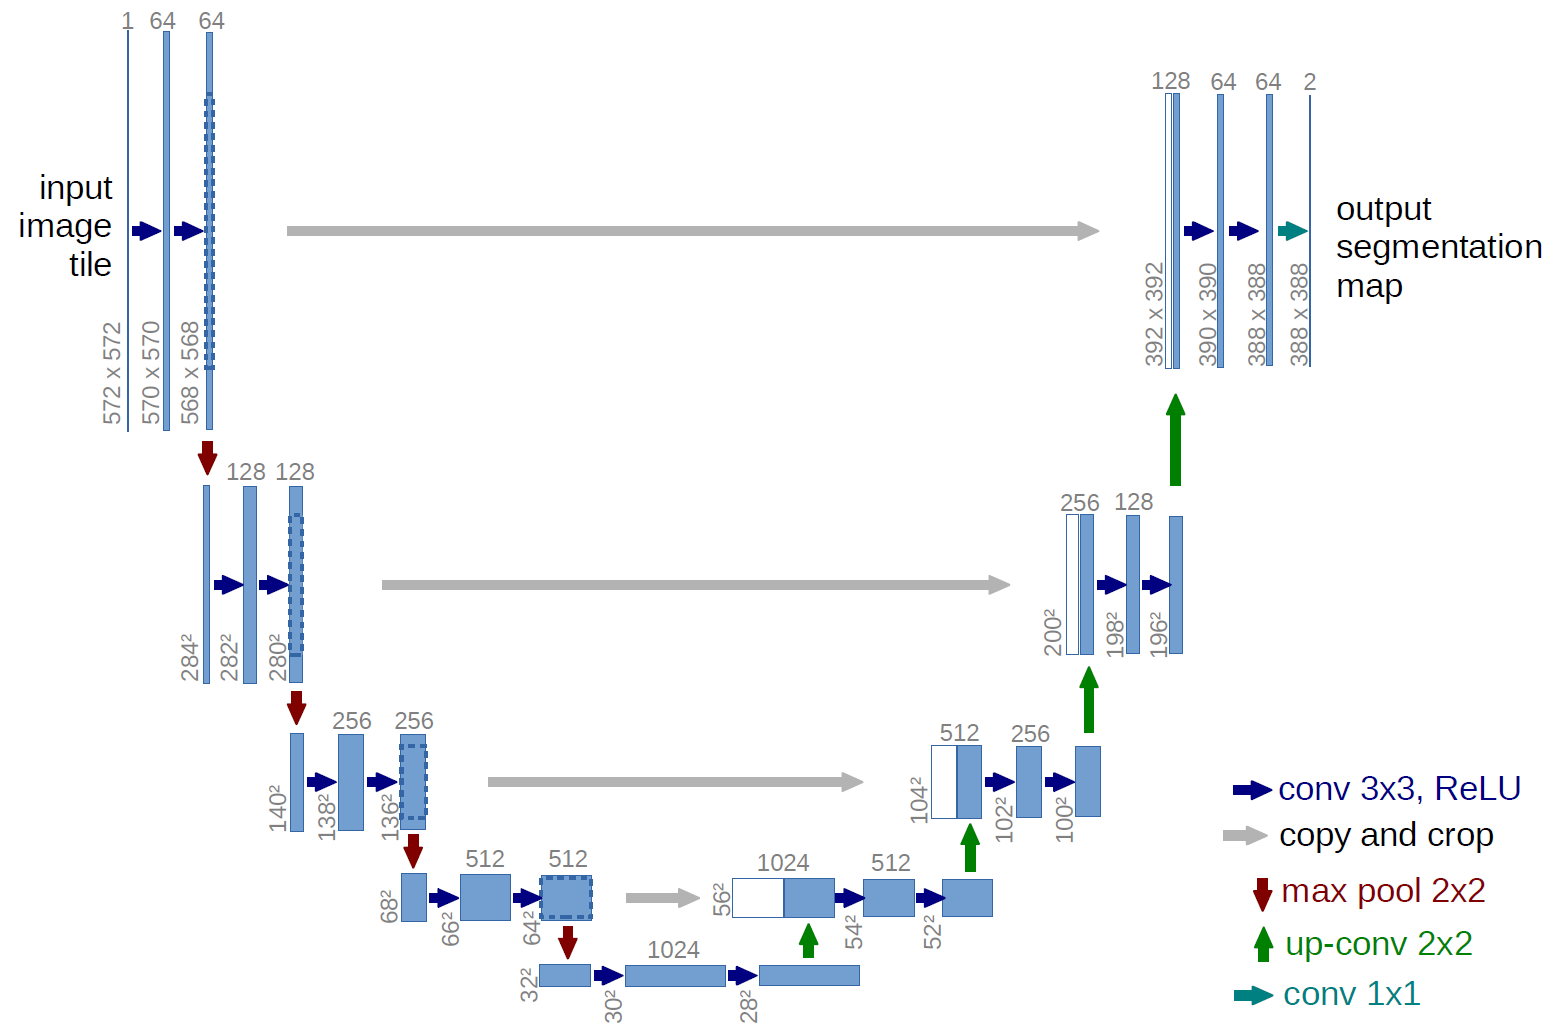
\includegraphics[width=\textwidth]{img/u-net-architecture.png}
\caption{A generic U-Net Architecture}\label{fig:unet}
\end{figure}

\vfill\null\newpage
The U-Net Architecture have these following properties that enables it perform well on assigning classes to each pixel: 

\begin{itemize}
    \item Multilevel Decomposition: For shrinking image sizes,  it utilizes the same size of convolutional kernels. In other words, for convolution, it employs different Fourier transform sizes to match different images size allowing it to decompose the image in multiple different spatial frequencies. 
    \item Residual Learning: The skip connections created in between input and output, along with the encoded features in the encoder pathway and the decoded image from latent features, helps the model to learn also from the features encoded before the latent representation and speeds up the training and provide a good convergence rate, avoiding the vanishing gradient problem, borrowing the idea that was proposed for ResNet in \cite{he2016deep}. 
\end{itemize}

Thanks to the multichannel filtering feature of the CNNs, U-Net outputs usually more than one channels corresponding to foreground (with the segmentation class counts)
and the background. Using a proper cost function, such as mean squared error and an appropriate optimizer, the model learn the function that maps the pixels to the classification labels.  

\subsection{Attention}

Attention was first proposed for sequence-to-sequence tasks, such as machine translation. Since it is developed for natural language processing, its mechanism is illustrated using "words". In tasks, such as machine translation, the input's contextual location or the other words in the sentence might have a huge effect on the input, as in \Cref{fig:attention}, where the word "it" refers to two different words although it is in the same location in the sentence. However, what it refers is changed by the global dependency. In other words, the word at the very end of the sentence had an impact on the word itself. Hence, the ceontextual similarity should also be learned when training sequence-to-sequence models. 
\begin{figure}[h]
\centering
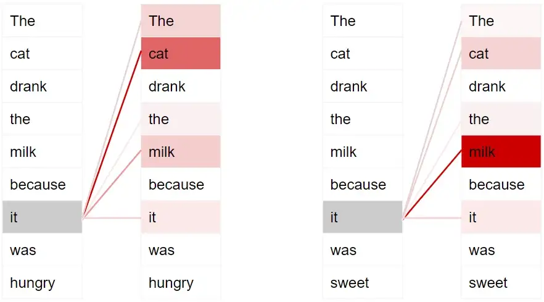
\includegraphics[width=\textwidth]{img/attention.png}
\caption{Words' contextual relation in the sentence \cite{doshi_2021}}\label{fig:attention}
\end{figure}

\vfill\null\newpage
To learn such relationship, the following mechanism is proposed: 
\begin{figure}[h]
\centering
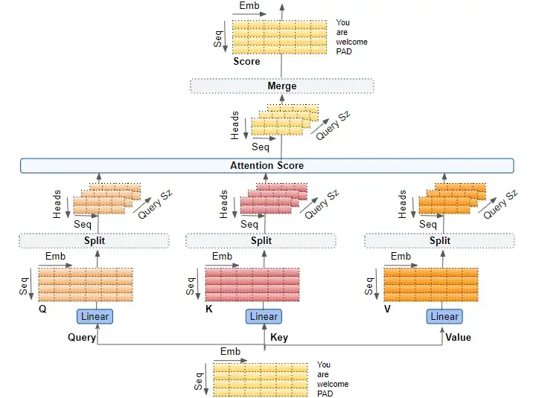
\includegraphics[width=0.8\textwidth]{img/attmech.png}
\caption{MultiHead Self Attention Mechanism}\label{fig:attmech}
\end{figure}

In \Cref{fig:attmech}, the sentence "You are welcome." is padded by one word and the words are transformed into vectors, or embedding, via an embedding network such as Word2Vec \cite{mikolov2013efficient}. In this example the embedding size is 6. Then, the embedding are transformed by some trainable linear transformations, or matrices $W_Q, W_K, W_V$, to three difference spaces, \textbf{Query}, \textbf{Key} and \textbf{Value}. Following this operation, the projections are splitted into different attention heads and the relationship weights are calculated using $\sigma(QK^T)$ where $\sigma$ is softmax. The weights corresponding to the \texttt{PAD} values are masked out and the resultant matrix is multiplied with matrix $V = W_vE$ where $E$ is the input embeddings to obtain the attention score. The multihead attention splits the transformed embedding and provides an opportunity for different part of embedding to learn different relations. For instance, one part of the embedding can encode the gender(in languages with gender pronouns) and other part of the embedding can encode the cardinality(singular or plural). 


\subsection{Extending Attention to Vision} \label{sec:vit}
One of the main works whose results were utilized in the study is Vision Transformer proposed in \cite{dosovitskiy2020image}.

\begin{figure}[h]
    \centering
    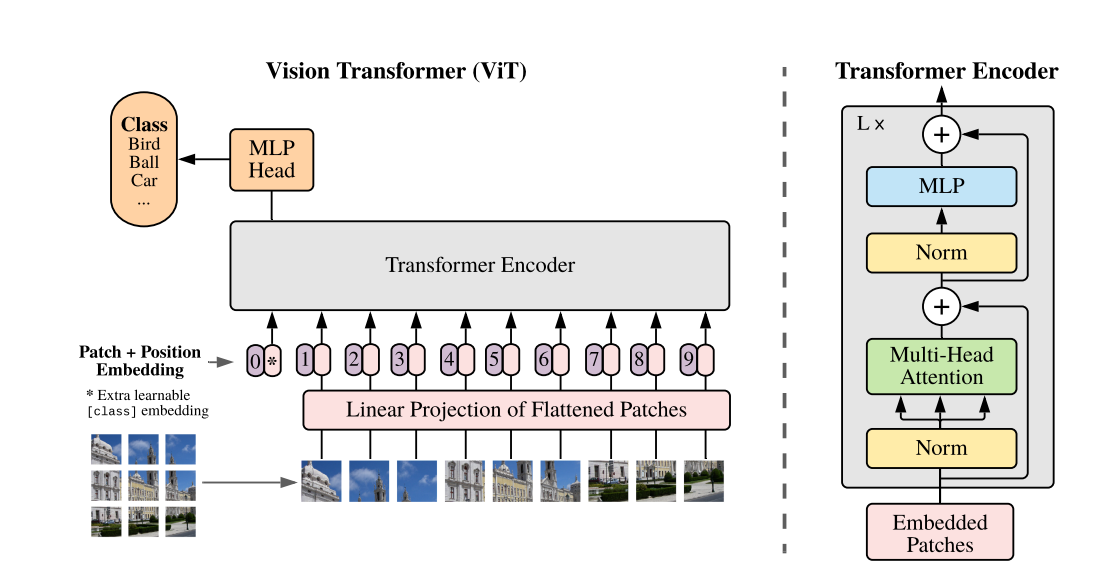
\includegraphics[width=\textwidth]{img/ViT.png}
    \caption{Vision Transformer}\label{fig:vit}
\end{figure}

\begin{figure*}[h]
    \centering
    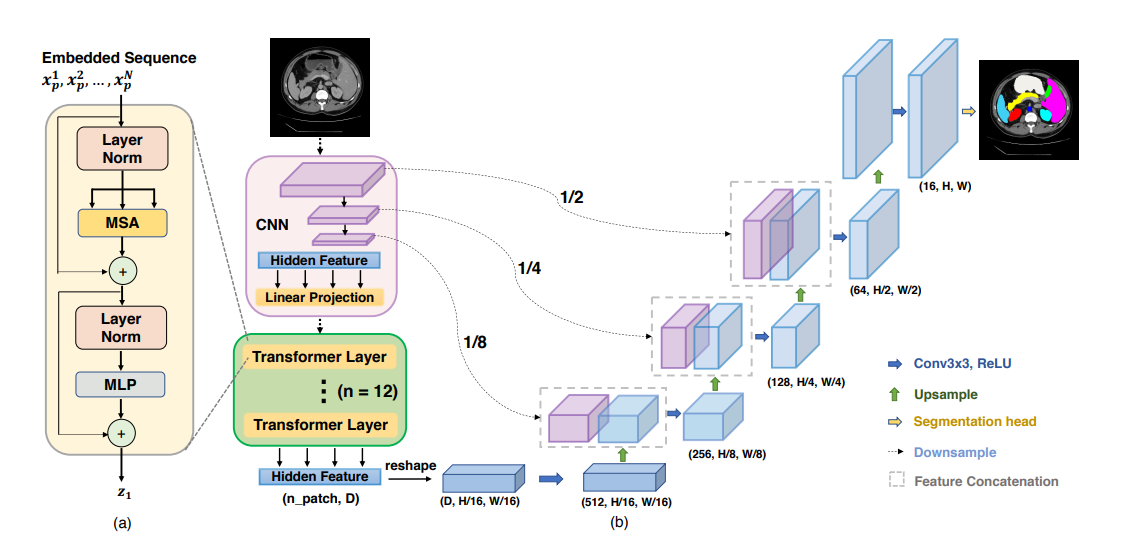
\includegraphics[width=\textwidth]{img/transunet.png}
    \caption{TransUnet Framework}\label{fig:tunet}
\end{figure*}

In the overview of this model we observe that image is splitted into fixed-size patches and are projected linearly after flattening, with an extra positional embedding. After linear projections, these embedding are fed into a transformer encoder which includes batch normalization, multihead attention, a multilayer perceptron and 2 skip-connections. By replacing the word embeddings with flattened image patches, Dosovitskiy \textit{et al.} was able to perform classification on the images.   

\subsection{TransUNet}

\subsubsection{Hybrid Model}
TransUNet is a hybrid network that exploits the local feature encoding characteristics of CNNs and global feature encoding characteristics of the transformers at the same time. As a modification on \cite{dosovitskiy2020image}, TransUNet employs a CNN as a feature extractor to generate a feature map. Then, patch embedding is applied to $1 \times 1$ patches extracted from the CNN feature map instead of the raw images. 

The authors list 2 reasons for following this approach: 1) it allows the utilization of CNN feature map in the decoding path; and 2) it results in better performance when compared to the case the inputs are taken as raw images. 

\begin{equation}
    z_0 = [x_p^1E; x_p^2E; \hdots; x_p^NE] + E_{pos}
    \label{eq:firstinput}
\end{equation}

where $E$ is the patch embedding projection and $E_{pos}$ is the positional embedding. 
Once the input of the first transformer is layer obtained as described in \Cref{eq:firstinput}, the l-th layer output of the transformer can be written as follows: 

\begin{eqnarray}
    {z'}_l &= MSA(LN(z_{l-1})) + z_{l-1} \\
    z_l &= MLP(LN({z'}_l)) + {z'}_l
\end{eqnarray}
\vfill\null\newpage
\subsubsection{Cascaded Upsampler (CUP)}
The decoded feature representation $z_L \in \mathbb{R}^{\frac{HW}{P^2}} \times D$ is reshaped to $\frac{H}{P} \times \frac{W}{P}$. Then, by using 1$\times$1 convolution, the number of channels are reduced to number of classes. This approach directly applies bilinear upsampling (interpolation) on the coded representation and the resultant tensor is the output result. This na\"ive interpolation approac is called "None" in \cite{chen2021transunet}. Instead of this, the researchers cascade multiple upsampling blocks consisting of 2$\times$ upsampling operator, a $3\times 3$ convolution layer and ReLU nonlinearity successively. 

\subsection{Experiments and Results}

\subsubsection{Performance Metrics} 

The metrics defined in \Cref{eq:DC,eq:HD} are utilized for the evaluation of the performance.

\begin{align}
    Dice \ Coeff.(DSC) &= 2 \times \frac{A \cap B}{A \cup B} \label{eq:DC}\\
    d_H(X,Y) (HD) &= \max \left\{ \sup_{x\in X} d(x,Y),\sup_{b\in B} d(X,y) \right\} \label{eq:HD}
\end{align}

where $A$ and $B$ in \Cref{eq:DC} are target and found segmentation regions, whereas $X$ and $Y$ in \Cref{eq:HD}, the Hausdorff distance, are the segmentation boundaries corresponding to the segmented regions.

When the model predictions show exact match with labelled regions, both metrics are 1. 

\begin{figure*}[h]
\centering
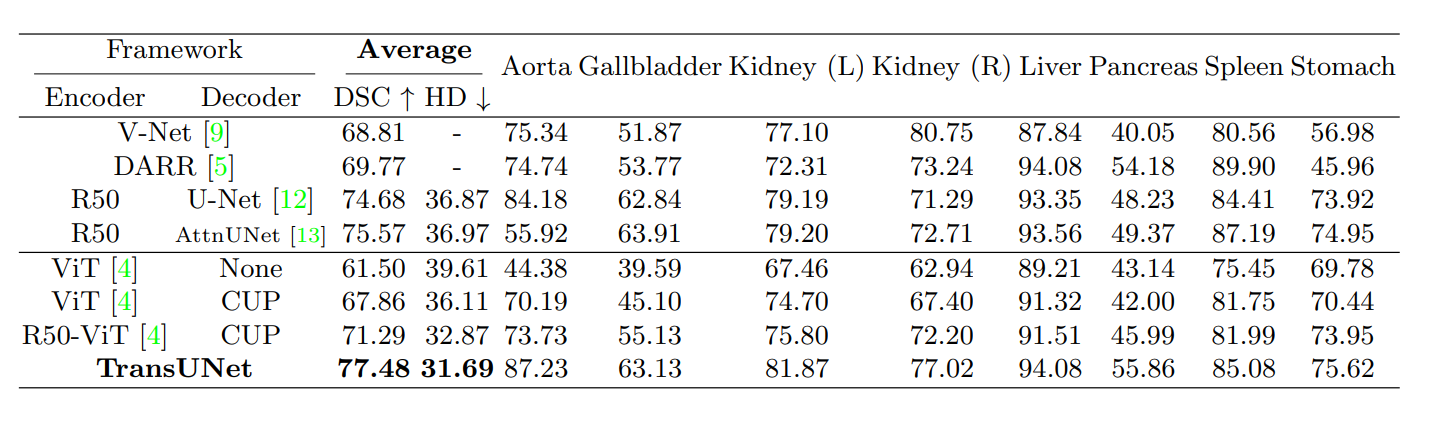
\includegraphics[width=0.8\textwidth]{img/table1.png}
\caption{Comparsion on SYNAPSE dataset}\label{fig:table}
\end{figure*}

\begin{figure*}[h]
\centering
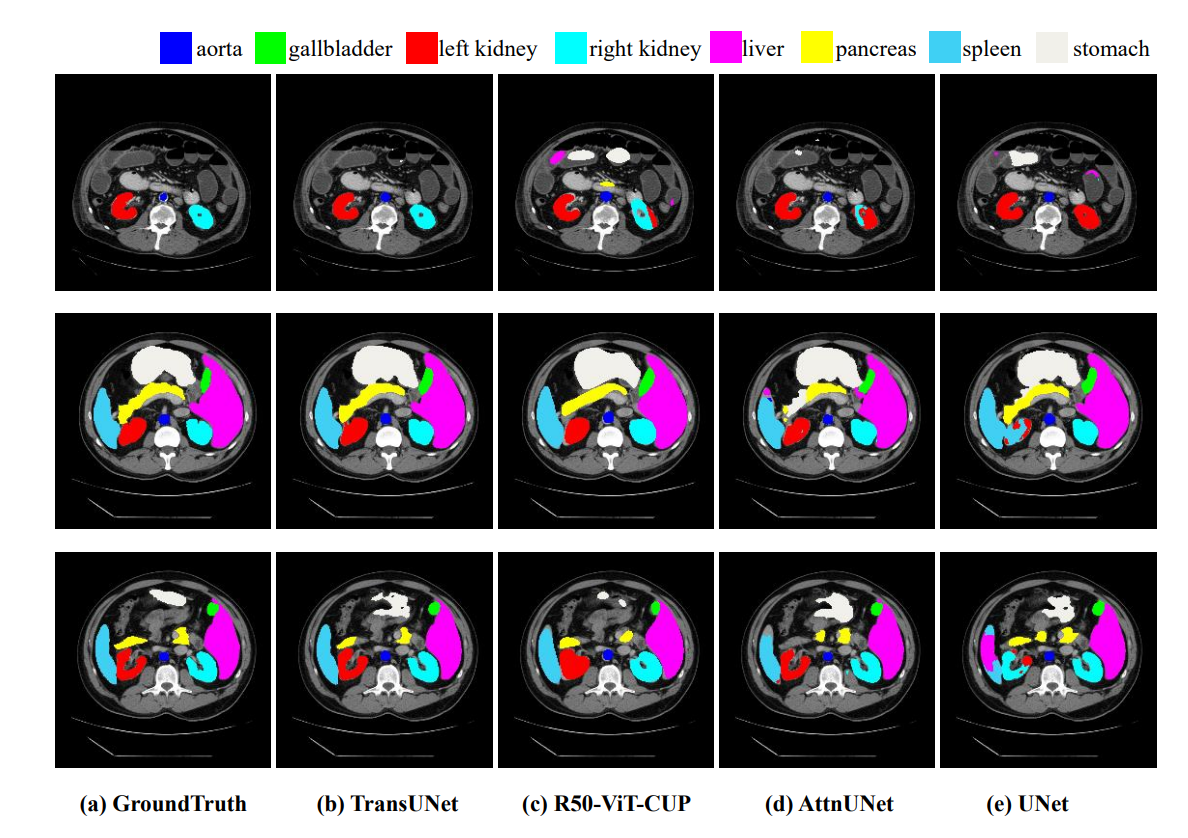
\includegraphics[width=0.8\textwidth]{img/results_qual.png}
\caption{Qualitative results for SYNAPSE dataset}\label{fig:synapseseg}
\end{figure*}

\vfill\null\newpage

\begin{table}[h]
\caption{Automated Cardiac Diagnosis Challenge dataset results}\label{tab:acdc}
\centering{
\begin{tabular}{|c|c|ccc|} \hline
    Framework & Average & RV & Myo & LV \\ \hline
    R50-U-Net & 87.55 & 87.10 & 80.63 & 94.62 \\
    R50-AttnUNet & 86.75 & 87.58 & 79.20 & 93.47\\
    ViT-CUP &81.45 &81.46 &70.71 &92.18\\
    R50-ViT-CUP &87.57 &86.07 &81.88 &94.75\\
    TransUNet &89.71 &88.86 &84.53 &95.73 \\ \hline
\end{tabular}}
\end{table}

\subsubsection{Original Results \cite{chen2021transunet}}

There are a series of ablation studies to determine the number of skip connections, input resolution, patch size and sequence length. The latter three are dependent on each other by the relation $P^2L = WH = W^2$, where $P$ is the patch size, $L$ is the sequence length and $W$ and $H$ is the input image sizes. To train the proposed network, Chen \textit{et al.} used 30 abdominal CT scans in the MICCAI 2015 Multi-Atlas Abdomen Labelling Challenge, adding up to 3779 axial contrast-enhanced images from SYNAPSE dataset and ACDC dataset. The experiments are done with different encoder and decoder architectures and the average DSC in percentage and Hausdorff distance in millimeters for eight abdominal organs with a random split 18 training and 12 validation cases are reported. Looking at \Cref{fig:table}, we see that TransUNet outperforms the best predecessor by 2.8\% in terms of average DSC and it reduced the HD by approximately 3\% when compared with the best predecessor. It is possible to investigate that the proposed method's performance is the best for 4 organs presented in \Cref{fig:table}. In \Cref{tab:acdc}, we observe that for both metrics, TransUNet outperformed the others for segmentation classes Left Ventricle, Myocardium and Right Ventricle.
\vfill\null\newpage
\paragraph{Implementation details and training setup}
The models are trained on a single Nvidia RTX2080Ti GPU with following hyperparameters:
\begin{itemize}
    \item Input size: 224 $\times$ 224
    \item Patch size: 16
    \item Learning rate: 0.01
    \item Momentum 0.9 
    \item Weight decay: 0.0001
    \item Optimizer: Sthocastic Gradient Descent
    \item Number of training iterations: 20000
    \item Default batch size: 24
\end{itemize}



\clearpage
\printbibliography{}
\end{document}

